\documentclass[12pt]{article}

\usepackage{amsmath, mathtools}
\usepackage{amsfonts}
\usepackage{amssymb}
\usepackage{graphicx}
\usepackage{colortbl}
\usepackage{xr}
\usepackage{hyperref}
\usepackage{longtable}
\usepackage{xfrac}
\usepackage{tabularx}
\usepackage{float}
\usepackage{siunitx}
\usepackage{booktabs}
\usepackage{caption}
\usepackage{pdflscape}
\usepackage{afterpage}

%\usepackage[round]{natbib}

%\usepackage{refcheck}

\hypersetup{
    bookmarks=true,         % show bookmarks bar?
      colorlinks=true,       % false: boxed links; true: colored links
    linkcolor=red,          % color of internal links (change box color with linkbordercolor)
    citecolor=green,        % color of links to bibliography
    filecolor=magenta,      % color of file links
    urlcolor=cyan           % color of external links
}

%% Comments

\usepackage{color}

\newif\ifcomments\commentstrue %displays comments
%\newif\ifcomments\commentsfalse %so that comments do not display

\ifcomments
\newcommand{\authornote}[3]{\textcolor{#1}{[#3 ---#2]}}
\newcommand{\todo}[1]{\textcolor{red}{[TODO: #1]}}
\else
\newcommand{\authornote}[3]{}
\newcommand{\todo}[1]{}
\fi

\newcommand{\wss}[1]{\authornote{blue}{SS}{#1}} 
\newcommand{\plt}[1]{\authornote{magenta}{TPLT}{#1}} %For explanation of the template
\newcommand{\an}[1]{\authornote{cyan}{Author}{#1}}

%% Common Parts

\newcommand{\progname}{Mechatronics Engineering} % PUT YOUR PROGRAM NAME HERE
\newcommand{\authname}{Team 10, LiDart
\\ Jonathan Casella
\\ Karim Elmokattaf
\\ Michaela Schnull
\\ Neeraj Ahluwalia} % AUTHOR NAMES                  

\usepackage{hyperref}
    \hypersetup{colorlinks=true, linkcolor=blue, citecolor=blue, filecolor=blue,
                urlcolor=blue, unicode=false}
    \urlstyle{same}
                                


% For easy change of table widths
\newcommand{\colZwidth}{1.0\textwidth}
\newcommand{\colAwidth}{0.13\textwidth}
\newcommand{\colBwidth}{0.82\textwidth}
\newcommand{\colCwidth}{0.1\textwidth}
\newcommand{\colDwidth}{0.05\textwidth}
\newcommand{\colEwidth}{0.8\textwidth}
\newcommand{\colFwidth}{0.17\textwidth}
\newcommand{\colGwidth}{0.5\textwidth}
\newcommand{\colHwidth}{0.28\textwidth}

% Used so that cross-references have a meaningful prefix
\newcounter{defnum} %Definition Number
\newcommand{\dthedefnum}{GD\thedefnum}
\newcommand{\dref}[1]{GD\ref{#1}}
\newcounter{datadefnum} %Datadefinition Number
\newcommand{\ddthedatadefnum}{DD\thedatadefnum}
\newcommand{\ddref}[1]{DD\ref{#1}}
\newcounter{theorynum} %Theory Number
\newcommand{\tthetheorynum}{T\thetheorynum}
\newcommand{\tref}[1]{T\ref{#1}}
\newcounter{tablenum} %Table Number
\newcommand{\tbthetablenum}{T\thetablenum}
\newcommand{\tbref}[1]{TB\ref{#1}}
\newcounter{assumpnum} %Assumption Number
\newcommand{\atheassumpnum}{P\theassumpnum}
\newcommand{\aref}[1]{A\ref{#1}}
\newcounter{goalnum} %Goal Number
\newcommand{\gthegoalnum}{P\thegoalnum}
\newcommand{\gsref}[1]{GS\ref{#1}}
\newcounter{instnum} %Instance Number
\newcommand{\itheinstnum}{IM\theinstnum}
\newcommand{\iref}[1]{IM\ref{#1}}
\newcounter{reqnum} %Requirement Number
\newcommand{\rthereqnum}{P\thereqnum}
\newcommand{\rref}[1]{R\ref{#1}}
\newcounter{nfrnum} %NFR Number
\newcommand{\rthenfrnum}{NFR\thenfrnum}
\newcommand{\nfrref}[1]{NFR\ref{#1}}
\newcounter{lcnum} %Likely change number
\newcommand{\lthelcnum}{LC\thelcnum}
\newcommand{\lcref}[1]{LC\ref{#1}}

\newcommand{\RobotSpeed}{0.5m/s}
\newcommand{\ScanTolerance}{+/- 1cm}
\newcommand{\BatteryLife}{3hrs}
\newcommand{\ScanningSpace}{1 square meter}
\newcommand{\ScanningTime}{2mins}
\newcommand{\MaxProcessingTime}{10mins}
\newcommand{\MaxResponseTime}{1s}
\newcommand{\MinVideoResolution}{1280x720}
\newcommand{\MaxVideoDelay}{1s}
\newcommand{\RobotMaxWeight}{50kg}
\newcommand{\RobotMaxDimensions}{1m x 1m x 3m (LxWxH)}
\newcommand{\MaxNavLevels}{4}
\newcommand{\MinFontSize}{14pt}
\newcommand{\ExecuteTaskTime}{10s}

\usepackage{fullpage}

\newcommand{\deftheory}[9][Not Applicable]
{
\newpage
\noindent \rule{\textwidth}{0.5mm}

\paragraph{RefName: } \textbf{#2} \phantomsection 
\label{#2}

\paragraph{Label:} #3

\noindent \rule{\textwidth}{0.5mm}

\paragraph{Equation:}

#4

\paragraph{Description:}

#5

\paragraph{Notes:}

#6

\paragraph{Source:}

#7

\paragraph{Ref.\ By:}

#8

\paragraph{Preconditions for \hyperref[#2]{#2}:}
\label{#2_precond}

#9

\paragraph{Derivation for \hyperref[#2]{#2}:}
\label{#2_deriv}

#1

\noindent \rule{\textwidth}{0.5mm}

}

\begin{document}

\title{Software Requirements Specification\\
\progname} 
\author{\authname}
\date{\today}
	
\maketitle

~\newpage

\pagenumbering{roman}

\tableofcontents

~\newpage

\section*{Revision History}

\begin{tabularx}{\textwidth}{p{3cm}p{2cm}p{4cm}X}
\toprule {\bf Date} & {\bf Version} & {\bf Authors} & {\bf Notes}\\
\midrule
05\textbackslash Oct\textbackslash 2022 & 1.0 & Michaela Schnull \newline Jonathan Casella \newline Kareem Elmokattaf \newline Neeraj Ahluwalia & Initial Release\\
\bottomrule
\end{tabularx}

~\newpage

\section{Reference Material}

This section records information for easy reference.

\subsection{Table of Units}

Throughout this document SI (Syst\`{e}me International d'Unit\'{e}s) is employed
as the unit system.  In addition to the basic units, several derived units are
used as described below.  For each unit, the symbol is given followed by a
description of the unit and the SI name.
~\newline

\renewcommand{\arraystretch}{1.2}
%\begin{table}[ht]
  \noindent \begin{tabular}{l l l} 
    \toprule		
    \textbf{symbol} & \textbf{unit} & \textbf{SI}\\
    \midrule 
    \si{\metre} & length & metre\\
    \si{\kilogram} & mass	& kilogram\\
    \si{\second} & time & second\\
    \si{\watt} & power & watt (W = \si{\joule\per\second})\\
    \bottomrule
  \end{tabular}
  %	\caption{Provide a caption}
%\end{table}

\plt{Only include the units that your SRS actually uses.}

\plt{Derived units, like newtons, pascal, etc, should show their derivation
    (the units they are derived from) if their constituent units are in the
    table of units (that is, if the units they are derived from are used in the
    document).  For instance, the derivation of pascals as
    $\si{\pascal}=\si{\newton\per\square\meter}$ is shown if newtons and m are
    both in the table.  The derivations of newtons would not be shown if kg and
    s are not both in the table.}

\plt{The symbol for units named after people use capital letters, but the name
  of the unit itself uses lower case.  For instance, pascals use the symbol Pa,
  watts use the symbol W, teslas use the symbol T, newtons use the symbol N,
  etc.  The one exception to this is degree Celsius.  Details on writing metric
  units can be found on the 
  \href{https://www.nist.gov/pml/weights-and-measures/writing-metric-units}
  {NIST} web-page.}

\subsection{Abbreviations and Acronyms}

\renewcommand{\arraystretch}{1.2}
\begin{tabular}{l l} 
  \toprule		
  \textbf{symbol} & \textbf{description}\\
  \midrule 
  A & Assumption\\
  CAD & Computer Aided Design\\
  CMM & Coordinate Measuring Machine\\
  FSM & Finite State Machine\\
  GS & Goal Statement\\
  GUI & Graphical User Interface\\
  IM & Instance Model\\
  LiDAR & Light Imaging, Detection, and Ranging\\
  LC & Likely Change\\
  NFR & Nonfunctional Requirement\\
  R & Requirement\\
  RAM & Random Access Memory\\
  SRS & System Requirements Specification\\
  VR & Virtual Reality\\
  \bottomrule
\end{tabular}\\

\plt{Add any other abbreviations or acronyms that you add}

\subsection{Terminology and  Definitions}

\begin{tabularx}{\textwidth}{p{3cm}X}
\toprule {\bf Term} & {\bf Definition}\\
\midrule
Term & Definition\\
\bottomrule
\end{tabularx}

\newpage

\pagenumbering{arabic}

\plt{This SRS template is based on {SmithAndLai2005, SmithEtAl2007}.  It
  will get you started.  You should not modify the section headings, without
  first discussing the change with the course instructor.  Modification means
  you are not following the template, which loses some of the advantage of a
  template, especially standardization.  Although the bits shown below do not
  include type information, you may need to add this information for your
  problem.  If you are unsure, please can ask the instructor.}

\plt{Feel free to change the appearance of the report by modifying the LaTeX
  commands.}

\plt{This template document assumes that a single program is being documented.
  If you are documenting a family of models, you should start with a commonality
  analysis.  A separate template is provided for this.  For program
  families you should look at \cite{Smith2006, SmithMcCutchanAndCarette2017}.
  Single family member programs are often programs based on a single physical
  model.  General purpose tools are usually documented as a family.  Families of
  physical models also come up.}

\plt{The SRS is not generally written, or read, sequentially.  The SRS is a
  reference document.  It is generally read in an ad hoc order, as the need
  arises.  For writing an SRS, and for reading one for the first time, the
  suggested order of sections is:
\begin{itemize}
\item Goal Statement
\item Instance Models
\item Requirements
\item Introduction
\item Specific System Description
\end{itemize}
}

\plt{Guiding principles for the SRS document:
\begin{itemize}
\item Do not repeat the same information at the same abstraction level.  If
  information is repeated, the repetition should be at a different abstraction
  level.  For instance, there will be overlap between the scope section and the
  assumptions, but the scope section will not go into as much detail as the
  assumptions section.
\end{itemize}
}

\plt{The template description comments should be disabled before submitting this
  document for grading.}

\plt{You can borrow any wording from the text given in the template.  It is part
  of the template, and not considered an instance of academic integrity.  Of
  course, you need to cite the source of the template.}

\plt{When the documentation is done, it should be possible to trace back to the
  source of every piece of information.  Some information will come from
  external sources, like terminology.  Other information will be derived, like
  General Definitions.}

\plt{An SRS document should have the following qualities: unambiguous,
  consistent, complete, validatable, abstract and traceable.}

\plt{The overall goal of the SRS is that someone that meets the Characteristics
  of the Intended Reader (Section~\ref{sec_IntendedReader}) can learn,
  understand and verify the captured domain knowledge.  They should not have to
  trust the authors of the SRS on any statements.  They should be able to
  independently verify/derive every statement made.}

\section{Introduction}

\plt{The introduction section is written to introduce the problem.  It starts general and focuses on the problem domain. The general advice is to start with a paragraph or two that describes the problem, followed by a ``roadmap'' paragraph.  A roadmap orients the reader by telling them what sub-sections to expect in the Introduction section.}

Businesses and individuals are increasingly using 3D scanning technologies to collect 3D data for modeling and analysis. The 3D scanning market is rapidly growing, with a wide range of applications such as VR, rapid prototyping, reverse-engineering, and inspection technologies. Many current scanning technologies require that objects are brought to specialized scanning facilities, where fixed devices such as CMM machines and robotic arms are installed. Hand-held scanning devices are also available,  however these technologies are expensive and require human operation. The cost and domain specific knowledge required are barriers to many users. There are limited solutions available for portable, remotely operated, and inexpensive 3D scanning solutions.  A low cost, portable, and user-friendly scanning solution would make scanning accessible to a wider audience.
\newline
\par
This document defines the scope of the \progname\ project, specifies the scanning system, and defines requirements. The purpose of the SRS is discussed in detail in Section~\ref{sec_purpose}.  Section~\ref{sec_Scope} describes key project deliverables, as well as exclusions that are outside the scope of work. Readers of this document should be familiar with concepts outlined in Section~\ref{sec_IntendedReader}.

\subsection{Problem Description and Goals}

\subsection{Purpose of Document}
\label{sec_purpose}

\plt{This section summarizes the purpose of the SRS document.  It does not focus
  on the problem itself.  The problem is described in the ``Problem
  Description'' section (Section~\ref{Sec_pd}).  The purpose is for the document
  in the context of the project itself, not in the context of this course.
  Although the ``purpose'' of the document is to get a grade, you should not
  mention this.  Instead, ``fake it'' as if this is a real project.  The purpose
  section will be similar between projects.  The purpose of the document is the
  purpose of the SRS, including communication, planning for the design stage,
  etc.}
  
  The purpose of this document is to provide specifications and requirements for the \progname\ 3D scanning system. This document describes functional and non-functional requirements, undesired event handling, and start-up behavior. The functional behaviour of the system is modeled through system diagrams and instance models. The requirements defined in this document will drive design decisions and will be referenced throughout the design phase to ensure requirements are being met. The requirements will be a direct input to the verification and validation plan.

\subsection{Scope of Requirements} 
\label{sec_Scope}

\plt{Modelling the real world requires simplification.  The full complexity of
  the actual physics, chemistry, biology is too much for existing models, and
  for existing computational solution techniques.  Rather than say what is in
  the scope, it is usually easier to say what is not.  You can think of it as
  the scope is initially everything, and then it is constrained to create the
  actual scope.  For instance, the problem can be restricted to 2 dimensions, or
  it can ignore the effect of temperature (or pressure) on the material
  properties, etc.}  

\plt{The scope section is related to the assumptions section
  (Section~\ref{sec_assumpt}).  However, the scope and the assumptions are not
  at the same level of abstraction.  The scope is at a high level.  The focus is
  on the ``big picture'' assumptions.  The assumptions section lists, and
  describes, all of the assumptions.}

\progname\ aims to design and build a low cost 3D scanning robot, paired with a user application that displays a model of the scanned data. The robot is expected to operate indoors on flat surfaces in a controlled environment. A robot that is capable of operating outdoors or on rough terrain is not in the scope of this project. The user software application will allow users to view 3D data. However, tools for analyzing and modifying 3D models generated by the application will not be implemented. Software considerations such as licensing, user authentication, security, and data storage are also not within the scope of this project.

\subsection{Organization of Document}

\plt{This section provides a roadmap of the SRS document.  It will help the
  reader orient themselves.  It will provide direction that will help them
  select which sections they want to read, and in what order.  This section will
  be similar between project.}
The rest of this document provides detailed specifications and requirements for the \progname\ 3D scanning system. The document is organized as follows:  
  
\noindent \begin{description}
\item Section~\ref{sec_GeneralDesc}: General System Description 
\newline
A general overview of the system is provided using a system context diagram. The interactions between the system, the environment,and its users are identified.
\item Section~\ref{sec_SpecificDesc}: Specific System Description 
\newline 
The problem description and project goals are given, followed by system specifications including assumptions, theories, definitions, and instance models.
\item Section~\ref{sec_Requirements}: Requirements
\newline
This section defines the functional and non-functional requirements of the system.
\item Section~\ref{sec_LikelyChanges}: Likely Changes
\newline
This section describes changes to system components that are likely to occur as a result of new features or changes in scope.
\item Section~\ref{sec_UnlikelyChanges}: Unlikely Changes 
\newline
This section describes the system requirements that are not likely to change.
\item Section~\ref{sec_dp}: Development Plan 
\newline
A plan outlining the steps that will be taken to create the \progname\ system is given.
\item Section~\ref{sec_ac}: Values of Auxiliary Constants 
\newline
This section provides values for symbolic parameters used in this document.
\end{description}

\section{General System Description} 
\label{sec_GeneralDesc}

This section provides general information about the system.  It identifies the
interfaces between the system and its environment, describes the user
characteristics and lists the system constraints.  \plt{This text can likely be
  borrowed verbatim.}

\plt{The purpose of this section is to provide general information about the
  system so the specific requirements in the next section will be easier to
  understand. The general system description section is designed to be
  changeable independent of changes to the functional requirements documented in
  the specific system description. The general system description provides a
  context for a family of related models.  The general description can stay the
  same, while specific details are changed between family members.}

\subsection{System Context}

\plt{Your system context will include a figure that shows the abstract view of
  the software.  Often in a scientific context, the program can be viewed
  abstractly following the design pattern of Inputs $\rightarrow$ Calculations
  $\rightarrow$ Outputs.  The system context will therefore often follow this
  pattern.  The user provides inputs, the system does the calculations, and then
  provides the outputs to the user.  The figure should not show all of the
  inputs, just an abstract view of the main categories of inputs (like material
  properties, geometry, etc.).  Likewise, the outputs should be presented from
  an abstract point of view.  In some cases the diagram will show other external
  entities, besides the user.  For instance, when the software product is a
  library, the user will be another software program, not an actual end user.
  If there are system constraints that the software must work with external
  libraries, these libraries can also be shown on the System Context diagram.
  They should only be named with a specific library name if this is required by
  the system constraint.}
  
Figure~\ref{Fig_SystemContext} is a system context diagram of the \progname\ 3D scanning system.

\begin{figure}[H]
\begin{center}
 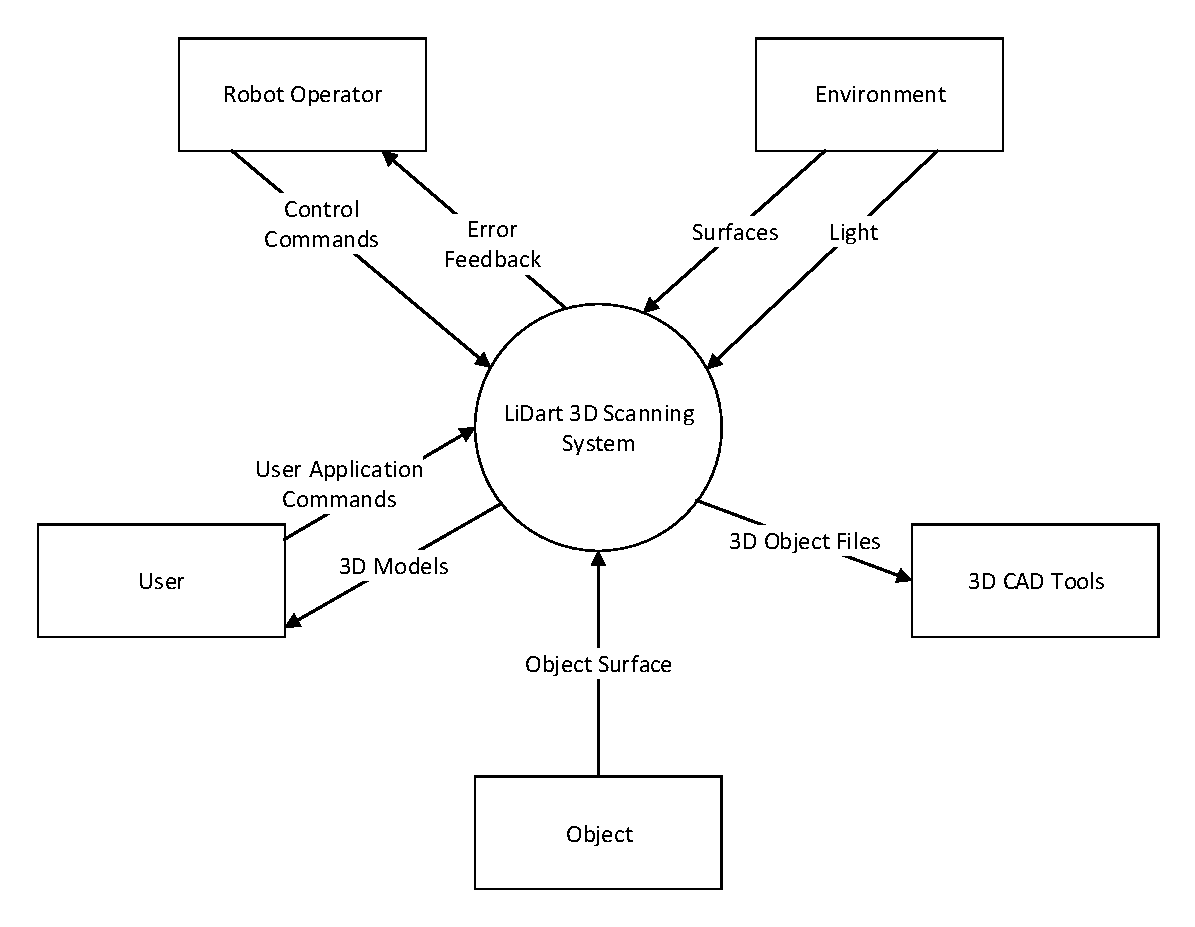
\includegraphics[width=0.9\textwidth]{Figures/Context Diagram.pdf}
\caption{System Context Diagram}
\label{Fig_SystemContext} 
\end{center}
\end{figure}

\plt{For each of the entities in the system context diagram its responsibilities
  should be listed.  Whenever possible the system should check for data quality,
  but for some cases the user will need to assume that responsibility.  The list
  of responsibilites should be about the inputs and outputs only, and they
  should be abstract.  Details should not be presented here.  However, the
  information should not be so abstract as to just say ``inputs'' and
  ``outputs''.  A summarizing phrase can be used to characterize the inputs.
  For instance, saying ``material properties'' provides some information, but it
  stays away from the detail of listing every required properties.}

\begin{itemize}
\item Robot Operator:
\begin{itemize}
\item The operator remotely controls the robot by sending commands to the robot. It is the operator's responsibility to instruct the robot to move and scan the desired object. 
\end{itemize}
\end{itemize}

\begin{itemize}
\item Environment:
\begin{itemize}
\item Information extracted from the surrounding environment is an input to the scanning system.
\end{itemize}
\end{itemize}

\begin{itemize}
\item User: 
\begin{itemize}
\item The user is responsible for providing input commands to the user application. 
\end{itemize}
\end{itemize}

\begin{itemize}
\item Object:
\begin{itemize}
\item The desired object that is being scanned is an input to the system.
\end{itemize}
\end{itemize}

\begin{itemize}
\item 3D CAD Tools:
\begin{itemize}
\item External 3D CAD tools are able to import 3D object files that are outputted by the \progname\ system. Further analysis and modification of 3D data can be carried out external CAD applications.
\end{itemize}
\end{itemize}

\begin{itemize}
\item \progname\ 3D Scanning System:
\begin{itemize}
\item The system will provide the robot operator with alerts about errors that occur during scanning operations.
\item The system is responsible for executing commands provided by the operator.
\item The system will check that the data it receives from the surrounding environment is valid.
\item The user application will respond to commands provided by the user.
\item The system outputs 3D Object Files that are supported by external CAD tools.
\item The user application will provide the user with view-able 3D models.
\end{itemize}
\end{itemize}

\subsection{User Characteristics} \label{SecUserCharacteristics}

\plt{This section summarizes the knowledge/skills expected of the user.
  Measuring usability, which is often a required non-function requirement,
  requires knowledge of a typical user.  As mentioned above, the user is a
  different role from the ``intended reader,'' as given in
  Section~\ref{sec_IntendedReader}.  As in Section~\ref{sec_IntendedReader}, the
  user characteristics should be specific an unambiguous.  For instance, ``The
  end user of \progname{} should have an understanding of undergraduate Level 1
  Calculus and Physics.''}
  
The \progname\ 3D scanning system does not require any domain specific knowledge. Individuals and business using the system are expected to have the following prior knowledge:   
  
\begin{itemize}
\item An understanding of how to install applications on personal computers
\item An understanding of 3D data file types and CAD programs
\item Basic computer skills, such as how to navigate through application menus
\end{itemize}

\subsection{System Constraints}

\plt{System constraints differ from other type of requirements because they
  limit the developers' options in the system design and they identify how the
  eventual system must fit into the world. This is the only place in the SRS
  where design decisions can be specified.  That is, the quality requirement for
  abstraction is relaxed here.  However, system constraints should only be
  included if they are truly required.}

The following constraints are imposed on the \progname\ system:
\begin{itemize}
\item The total cost of the system must be less than \$750.
\item Off-the-shelf, readily-available hardware shall be used where possible.

\end{itemize}

\section{Specific System Description} 
\label{sec_SpecificDesc}

This section presents assumptions, required behaviour, and a functional decomposition of the system.  

\subsection{Solution Characteristics Specification}

\plt{This section specifies the information in the solution domain of the system
  to be developed. This section is intended to express what is required in
  such a way that analysts and stakeholders get a clear picture, and the
  latter will accept it. The purpose of this section is to reduce the problem
  into one expressed in mathematical terms. Mathematical expertise is used to
  extract the essentials from the underlying physical description of the
  problem, and to collect and substantiate all physical data pertinent to the
  problem.}

\plt{This section presents the solution characteristics by successively refining
  models.  It starts with the abstract/general Theoretical Models (TMs) and
  refines them to the concrete/specific Instance Models (IMs).  If necessary
  there are intermediate refinements to General Definitions (GDs).  All of these
  refinements can potentially use Assumptions (A) and Data Definitions (DD).
  TMs are refined to create new models, that are called GMs or IMs. DDs are not
  refined; they are just used. GDs and IMs are derived, or refined, from other
  models. DDs are not derived; they are just given. TMs are also just given, but
  they are refined, not used.  If a potential DD includes a derivation, then
  that means it is refining other models, which would make it a GD or an IM.}

\plt{The above makes a distinction between ``refined'' and ``used.'' A model is
  refined to another model if it is changed by the refinement. When we change a
  general 3D equation to a 2D equation, we are making a refinement, by applying
  the assumption that the third dimension does not matter. If we use a
  definition, like the definition of density, we aren't refining, or changing
  that definition, we are just using it.}

\plt{The same information can be a TM in one problem and a DD in another.  It is
  about how the information is used.  In one problem the definition of
  acceleration can be a TM, in another it would be a DD.}

\plt{There is repetition between the information given in the different chunks
  (TM, GDs etc) with other information in the document.  For instance, the
  meaning of the symbols, the units etc are repeated.  This is so that the
  chunks can stand on their own when being read by a reviewer/user.  It also
  facilitates reuse of the models in a different context.}

\noindent \plt{The relationships between the parts of the document are show in
  the following figure.  In this diagram ``may ref'' has the same role as
  ``uses'' above.  The figure adds ``Likely Changes,'' which are able to
  reference (use) Assumptions.}

\begin{figure}[H]
  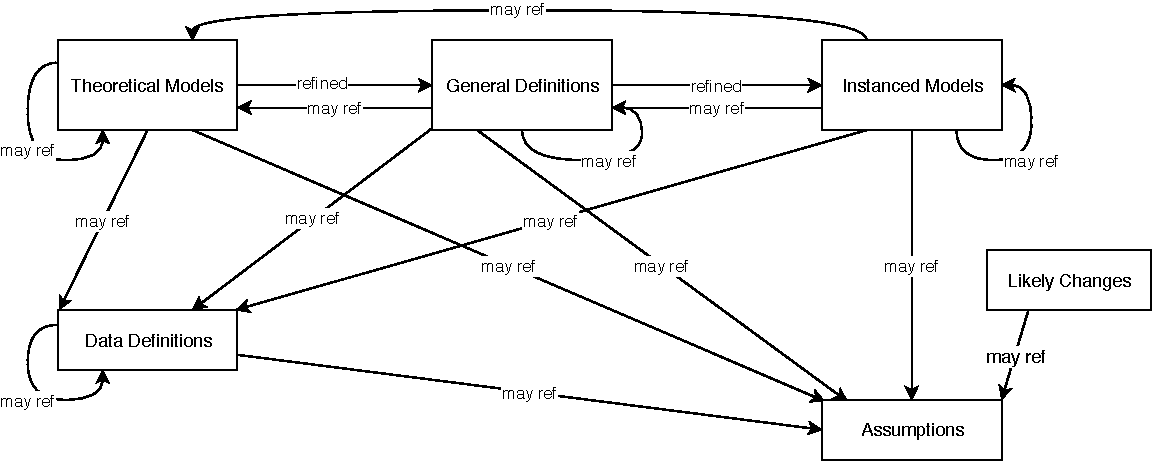
\includegraphics[scale=0.9]{RelationsBetweenTM_GD_IM_DD_A.pdf}
\end{figure}

The instance models that govern \progname{} are presented in
Subsection~\ref{sec_instance}.  The information to understand the meaning of the
instance models and their derivation is also presented, so that the instance
models can be verified.

\subsubsection{Assumptions} \label{sec_assumpt}

\plt{The assumptions are a refinement of the scope.  The scope is general, where
  the assumptions are specific.  All assumptions should be listed, even those
  that domain experts know so well that they are rarely (if ever) written down.}
\plt{The document should not take for granted that the reader knows which
  assumptions have been made. In the case of unusual assumptions, it is
  recommended that the documentation either include, or point to, an explanation
  and justification for the assumption.}

This section simplifies the original problem and helps in developing the
theoretical model by filling in the missing information for the physical
system. The numbers given in the square brackets refer to the theoretical model
[T], general definition [GD], data definition [DD], instance model [IM], or
likely change [LC], in which the respective assumption is used.

\begin{itemize}

\item[A\refstepcounter{assumpnum}\theassumpnum \label{A_meaningfulLabel}:]
  \plt{Short description of each assumption.  Each assumption
    should have a meaningful label.  Use cross-references to identify the
    appropriate traceability to T, GD, DD etc., using commands like dref, ddref
    etc.  Each assumption should be atomic - that is, there should not be an
    explicit (or implicit) ``and'' in the text of an assumption.}

\end{itemize}

\subsection{Behaviour Overview}\label{sec_behaviour}

\subsection{Functional Decomposition}\label{sec_behaviour}

\subsection{Subsystem Descriptions}\label{sec_behaviour}

\section{Requirements}
\label{sec_Requirements}

\plt{The requirements refine the goal statement.  They will make heavy use of
  references to the instance models.}

This section provides the functional requirements, the business tasks that the
software is expected to complete, and the nonfunctional requirements, the
qualities that the software is expected to exhibit.

\subsection{Functional Requirements}

\noindent \begin{itemize}

\item[R\refstepcounter{reqnum}\thereqnum \label{R_Inputs1}:] The system shall take input from the user through a keyboard and standard pointing device such as a mouse.
\item[R\refstepcounter{reqnum}\thereqnum \label{R_Inputs2}:] There shall be a kill-switch mounted on the robot, which immediately deactivates the the robot when pressed in emergency situations.
\item[R\refstepcounter{reqnum}\thereqnum \label{R_Inputs3}:] The robot shall be able to move in all four directions: turn left, turn right, move forwards, and move backwards.
\item[R\refstepcounter{reqnum}\thereqnum \label{R_Inputs4}:] The robot shall be stationary if no input commands are given.
<<<<<<< HEAD
\item[R\refstepcounter{reqnum}\thereqnum \label{R_Inputs5}:] The robot shall be able to be connected to over a wireless network.
\newline Rationale: A wireless connection is required for remote operation.
\item[R\refstepcounter{reqnum}\thereqnum \label{R_Inputs6}:] The robot shall be able to operated remotely.
=======
\item[R\refstepcounter{reqnum}\thereqnum \label{R_Inputs5}:] The robot shall be able to be connected to over Wifi.
\item[R\refstepcounter{reqnum}\thereqnum \label{R_Inputs6}:] The robot shall be able to be operated remotely.
>>>>>>> e72e2b9b3cb5f01454eed00802f6e5f918d20ffe
\item[R\refstepcounter{reqnum}\thereqnum \label{R_Inputs7}:] The robot shall have a power on/off switch.
\item[R\refstepcounter{reqnum}\thereqnum \label{R_Inputs8}:] The robot shall have a means of being charged.

\item[R\refstepcounter{reqnum}\thereqnum \label{R_OutputInputs1}:] The robot shall be able to verify the inputs before processing the output. (needs to be more specific)
\item[R\refstepcounter{reqnum}\thereqnum \label{R_Calculate1}:] The system shall be able to perform state estimation calculations based on landmarks in the surrounding environment.
\newline Rationale: 
\item[R\refstepcounter{reqnum}\thereqnum \label{R_Calculate2}:] The system shall calculate distance and rotation between each landmark.
\newline Rationale:
\item[R\refstepcounter{reqnum}\thereqnum \label{R_Calculate2}:] The system shall transform point-cloud data into a 3D object model.

\item[R\refstepcounter{reqnum}\thereqnum \label{R_VerifyOutput}:] The robot shall verify closed-loop calculations. (needs to be more specific)
\newline Rationale:

\item[R\refstepcounter{reqnum}\thereqnum \label{R_Output1}:] The GUI shall output the scanned data to a 3D model file type.
\newline Rationale: The exported files should be compatible with existing CAD applications.
\item[R\refstepcounter{reqnum}\thereqnum \label{R_Output2}:] The GUI shall display live video feed of the environment surrounding  the robot.
Rationale: This video feed can be used by the remote operator.
\item[R\refstepcounter{reqnum}\thereqnum \label{R_Output3}:] The GUI shall display a real-time visualization of the raw scanned data. 
\newline Rationale: A real-time representation of the data can be used by the robot operator to ensure the scanner is functioning properly.
\item[R\refstepcounter{reqnum}\thereqnum \label{R_Output4}:] The GUI shall display the current state of the system, as depicted in Figure~\ref{Fig_RobotFSM}.
\newline Rationale: The states can be used by the robot operator to troubleshoot operational issues.

\begin{figure}[H]
\begin{center}
 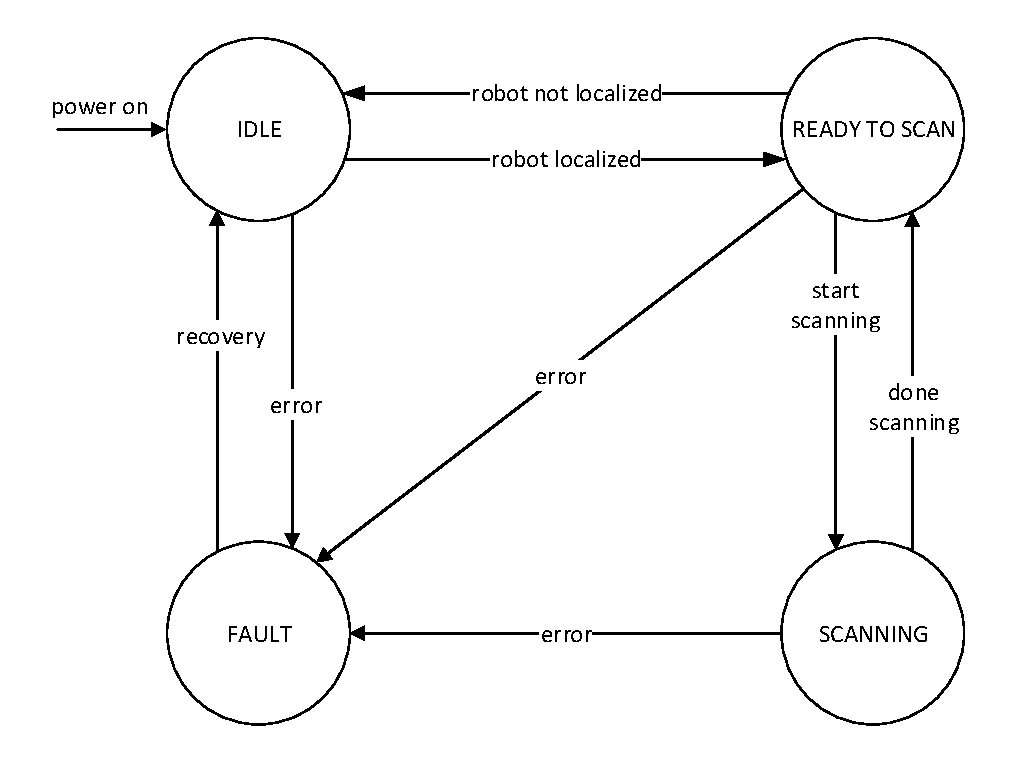
\includegraphics[width=0.75\textwidth]{Figures/Robot FSM.pdf}
\caption{Robot FSM}
\label{Fig_RobotFSM} 
\end{center}
\end{figure}
\end{itemize}

\subsection{Nonfunctional Requirements}

\plt{List your nonfunctional requirements.  You may consider using a fit criterion to make them verifiable.}
\plt{The goal is for the nonfunctional requirements to be unambiguous, abstract and verifiable.  This isn't easy to show succinctly, so a good strategy may be to give a ``high level'' view of the requirement, but allow for the details to be covered in the Verification and Validation document.}
\plt{An absolute requirement on a quality of the system is rarely needed.  For instance, an accuracy of 0.0101 \% is likely fine, even if the requirement is for 0.01 \% accuracy.  Therefore, the emphasis will often be more on describing now well the quality is achieved, through experimentation, and possibly theory, rather than meeting some bar that was defined a priori.}
\plt{You do not need an entry for correctness in your NFRs.  The purpose of the SRS is to record the requirements that need to be satisfied for correctness. Any statement of correctness would just be redundant. Rather than discuss correctness, you can characterize how far away from the correct (true) solution you are allowed to be.  This is discussed under accuracy.}

\subsubsection{Accuracy Requirements}
\plt{Characterize the accuracy by giving the context/use for the software.  Maybe something like, ``The accuracy of the computed solutions should meet the level needed for $<$engineering or scientific application$>$.  The level of accuracy achieved by \progname{} shall be described following the procedure given in Section~X of the Verification and Validation Plan.''  A link to the VnV plan would be a nice extra.}
    
\noindent \begin{itemize}
\item[NFR\refstepcounter{nfrnum}\thenfrnum\label{NFR_Accuracy1}:] The accuracy of the scans shall be within SCAN\_TOLERANCE. 
\newline Rationale: This level of accuracy meets the requirements needed for users of a low-cost, easily accessible scanning system.
\item[NFR\refstepcounter{nfrnum}\thenfrnum\label{NFR_Accuracy1}:] The accuracy of the scans shall be within \ScanTolerance{}. This level of accuracy meets the requirements needed for (insert application).
\end{itemize}

\subsubsection{Performance Requirements}

\noindent \begin{itemize}
\item[NFR\refstepcounter{nfrnum}\thenfrnum\label{NFR_Performance1}:] The robot shall be able to move at a maximum speed of \RobotSpeed{}.
\item[NFR\refstepcounter{nfrnum}\thenfrnum\label{NFR_Performance2}:] The robot shall be able to run for \BatteryLife{} of time without being charged.
\item[NFR\refstepcounter{nfrnum}\thenfrnum\label{NFR_Performance3}:] The system must be able to scan \ScanningSpace{} within \ScanningTime{} of time.
\item[NFR\refstepcounter{nfrnum}\thenfrnum\label{NFR_Performance4}:] The system shall require a maximum of \MaxProcessingTime{} to process raw data.
\item[NFR\refstepcounter{nfrnum}\thenfrnum\label{NFR_Performance5}:] The robot shall require a maximum of \MaxResponseTime{} to respond to user input commands.
\item[NFR\refstepcounter{nfrnum}\thenfrnum\label{NFR_Performance6}:] The video feed shall have a minimum resolution of \MinVideoResolution{}.

\item[NFR\refstepcounter{nfrnum}\thenfrnum\label{NFR_Performance7}:] The video feed displayed on the GUI shall have a maximum delay of \MaxVideoDelay{}.
\end{itemize}

\subsubsection{Usability Requirements}
\plt{Characterize the usability by giving the context/use for the software. You should likely reference the user characteristics section.  The level of usability achieved by the software shall be described following the procedure given in Section~X of the Verification and Validation Plan.  A link to the VnV plan would be a nice extra.}

\noindent \begin{itemize}
\item[NFR\refstepcounter{nfrnum}\thenfrnum \label{NFR_Usability1}:] The robot shall be easy to operate with very little knowledge. (needs to be measureable)
\item[NFR\refstepcounter{nfrnum}\thenfrnum \label{NFR_Usability2}:] The robot shall weigh less than \RobotMaxWeight{}.
\item[NFR\refstepcounter{nfrnum}\thenfrnum \label{NFR_Usability3}:] The robot shall be able to be stored within the dimensions \RobotMaxDimensions{}.
\item[NFR\refstepcounter{nfrnum}\thenfrnum \label{NFR_Usability4}:] The GUI shall be easy to navigate. The number of levels of navigation shall not exceed \MaxNavLevels{}.
\item[NFR\refstepcounter{nfrnum}\thenfrnum \label{NFR_Usability5}:] The font style and size shall be consistent throughout the GUI. Fonts must be sans-serif and have a minimum font size of \MinFontSize{}.
\item[NFR\refstepcounter{nfrnum}\thenfrnum \label{NFR_Usability6}:] The GUI shall be intuitive to use. Users must be able to execute desired tasks within \ExecuteTaskTime{} seconds of accessing the user interface, for at least every 9/10 tasks.
\end{itemize}

\subsubsection{Error-Handling Requirements}
\noindent \begin{itemize}
\item[NFR\refstepcounter{nfrnum}\thenfrnum \label{NFR_Errors1}:] The system shall display informative messages that alert the user of errors that have occurred. The messages may provide suggested steps to resolve the error.
\item[NFR\refstepcounter{nfrnum}\thenfrnum \label{NFR_Errors1}:] The system shall log error information. Error information should be specific and descriptive.
\end{itemize}

\subsubsection{Maintainability Requirements}
\plt{The effort required to make any of the likely changes listed for \progname{} should be less than FRACTION of the original development time.  FRACTION is then a symbolic constant that can be defined at the end of the report.}

\noindent \begin{itemize}
\item[NFR\refstepcounter{nfrnum}\thenfrnum \label{NFR_Maintainability1}:] Robot parts should be easily replaceable. It should take a maximum of 1 hour to replace any part on the robot.
\item[NFR\refstepcounter{nfrnum}\thenfrnum \label{NFR_Maintainability2}:] All hardware and electronic components shall be easily accessible. No special tools must be required to access hardware. 
\newline Rationale: This will facilitate activities such as debugging and reprogramming the robot. 
\item[NFR\refstepcounter{nfrnum}\thenfrnum \label{NFR_Maintainability2}:] Standard, off-the-shelf components shall be used where possible. 
\end{itemize}

\subsubsection{Portability Requirements}
\plt{This NFR is easier to write than the others.  The systems that \progname{} should run on should be listed here.  When possible the specific versions of the potential operating environments should be given.  To make the NFR verifiable a statement could be made that the tests from a given section of the VnV plan can be successfully run on all of the possible operating environments.}

\noindent \begin{itemize}
\item[NFR\refstepcounter{nfrnum}\thenfrnum \label{NFR_Portability1}:] The user application shall run on a Windows operating system.
\item[NFR\refstepcounter{nfrnum}\thenfrnum \label{NFR_Portability2}:] The user application must be able to run on a standard personal computer. For example, the application must be able to run on a system with an IntelCore i5 processor and 8 GB of RAM.
\end{itemize}

\subsubsection{Safety Requirements}
\noindent \begin{itemize}
\item[NFR\refstepcounter{nfrnum}\thenfrnum \label{NFR_Safety1}:] There shall not be any exposed electrical components or wiring.
\item[NFR\refstepcounter{nfrnum}\thenfrnum \label{NFR_Safety1}:] The operator shall be able to stop the robot at any time.
\item[NFR\refstepcounter{nfrnum}\thenfrnum \label{NFR_Safety2}:] The robot shall be placed in a safe-state if communication with the operator is lost.
\end{itemize}

\subsubsection{Standards Requirements}
\noindent \begin{itemize}
\item[NFR\refstepcounter{nfrnum}\thenfrnum \label{NFR_Safety2}:] The system shall be in conformace with the following standards:
\begin{itemize}
\item CSA 22.1:21, Canadian Electrical Code \cite{CSA1}
\item CSA Z434, Industrial robots and robot systems \cite{CSA2}
\end{itemize}
\end{itemize}

\section{Likely Changes} 
\label{sec_LikelyChanges}   

\noindent \begin{itemize}

\item[LC\refstepcounter{lcnum}\thelcnum\label{LC_meaningfulLabel}:] \plt{Give
    the likely changes, with a reference to the related assumption (aref), as appropriate.}

\end{itemize}

\section{Unlikely Changes} 
\label{sec_UnlikelyChanges} 

\noindent \begin{itemize}

\item[LC\refstepcounter{lcnum}\thelcnum\label{LC_meaningfulLabel}:] \plt{Give
    the unlikely changes.  The design can assume that the changes listed will
    not occur.}

\end{itemize}

\section{Development Plan}
\label{sec_dp}

\plt{This section is optional.  It is used to explain the plan for developing
  the software.  In particular, this section gives a list of the order in which
  the requirements will be implemented.  In the context of a course  this is
  where you can indicate which requirements will be implemented as part of the
  course, and which will be ``faked'' as future work.  This section can be
  organized as a prioritized list of requirements, or it could should the
  requirements that will be implemented for ``phase 1'', ``phase 2'', etc.}

\section{Values of Auxiliary Constants}
\label{sec_ac}

\plt{Show the values of the symbolic parameters introduced in the report.}

\plt{The definition of the requirements will likely call for SYMBOLIC\_CONSTANTS.
Their values are defined in this section for easy maintenance.}


\plt{The value of FRACTION, for the Maintainability NFR would be given here.}
\begin{tabular}{ | l | p{8cm} | c |}
  \hline
  \textbf{Constant} & \textbf{Description} & \textbf{Value} \\
  \hline
  RobotSpeed & Maximum speed of robot in navigation mode. & \RobotSpeed{} \\
  \hline
  ScanTolerance & Maximum deviation between sufficient scans. & \ScanTolerance{} \\
  \hline
  BatteryLife & Maximum time robot can run before needing to be recharged. & \BatteryLife{} \\
  \hline
  ScanningSpace & Unit used for defining robot scan speed & \ScanningSpace{} \\
  \hline
  ScanningTime & Time elapsed to complete scan of ScanningSpace. & \ScanningTime{} \\
  \hline
  MaxProcessingTime & Time needed for robot to process something. & \MaxProcessingTime{} \\
  \hline
  MaxResponseTime & Time needed for robot to respond to navigational commands given by user. & \MaxResponseTime{} \\
  \hline
  MinVideoResolution & Minimum resolution of video output feed in GUI. & \MinVideoResolution{} \\
  \hline
  MaxVideoDelay & Max time between change in camera and output video feed in GUI. & \MaxVideoDelay{} \\
  \hline
  RobotMaxWeight & Maximum weight of fully assembled robot. & \RobotMaxWeight{} \\
  \hline
  RobotMaxDimensions & Maximum size of fully assembled robot. & \RobotMaxDimensions{} \\
  \hline
  MaxNavLevels & Maximum number of layers required to access any function in GUI. & \MaxNavLevels{} \\
  \hline
  MinFontSize & The minimum font size used in the GUI for accessibility purposes. & \MinFontSize{} \\
  \hline
  ExecuteTaskTime & Time it would take an average user to execute 9/10 tasks within the GUI. & \ExecuteTaskTime{} \\
  \hline
  
\end{tabular}

\newpage
\nocite{*}
\bibliographystyle{ieeetr}
\bibliography{references}


\noindent \plt{The following is not part of the template, just some things to consider
  when filing in the template.}

\noindent \plt{Grammar, flow and \LaTeX advice:
\begin{itemize}
\item For Mac users \texttt{*.DS\_Store} should be in \texttt{.gitignore}
\item \LaTeX{} and formatting rules
\begin{itemize}
\item Variables are italic, everything else not, includes subscripts (link to
  document)
\begin{itemize}
\item \href{https://physics.nist.gov/cuu/pdf/typefaces.pdf}{Conventions}
\item Watch out for implied multiplication
\end{itemize}
\item Use BibTeX
\item Use cross-referencing
\end{itemize}
\item Grammar and writing rules
\begin{itemize}
\item Acronyms expanded on first usage (not just in table of acronyms)
\item ``In order to'' should be ``to''
\end{itemize}
\end{itemize}}

\noindent \plt{Advice on using the template:
\begin{itemize}
\item Difference between physical and software constraints
\item Properties of a correct solution means \emph{additional} properties, not
  a restating of the requirements (may be ``not applicable'' for your problem).
  If you have a table of output constraints, then these are properties of a
  correct solution.
\item Assumptions have to be invoked somewhere
\item ``Referenced by'' implies that there is an explicit reference
\item Think of traceability matrix, list of assumption invocations and list of
  reference by fields as automatically generatable
\item If you say the format of the output (plot, table etc), then your
  requirement could be more abstract
\end{itemize}
}

\newpage{}
\section*{Appendix --- Reflection}

	Throughout the LiDart project, the team will be collectively working on gaining knowledge as well as experience in order to get the project completed.  Ranging from programming to electrical to mechanical knowledge each team member will be gaining a lot of knowledge in their respective domains depending on their responsibilities.

Jon and Kareem will need to understand how to get the proper communication between the robot and the machine for the LIDAR sensors.
Throughout this process of figuring out the parameters, Jon will be able to expand on his knowledge on communications between the LIDAR sensors and the connected machine by working through the available documenation online. However, Kareem will be working on the controls of the robot by working through trial and error scenarios on the movement of the robot. Even though Kareem will be primarily working through trial and error, he will be using a lot of resources online to help learn how to properly figure out the routes of communication that are going to be used.
Jon has picked reading through online documentation since he prefers gathering information from the original source and then applying his understandings. Kareem has picked working through trial and error as that will be the best approach to seeing how the different parameters will affect the robot and its controls. Reading through documentation would not be very effective when trying to get the right controls for the robot as it would be based on theoretical values which won't directly apply to the robot. Through theory, values can be used as a starting point.

While the software is being configured, Neeraj will be working on making the chassi for the robot. Making the chassi for LiDart will require a lot of knowledge based on weight distribution and stabilizing the different moving components. The robot will have a variety of components such as the LIDAR sensors, mounting components and motors to name a few.
A lot of theory could be applied to designing the robot, but there will be a lot of trial and error with the process. That is why Neeraj is opting for using the trial and error method to figure out the best design for the robot. 

Lastly, the electrical components will be a very critical domain of the robot. Getting the correct electrical equipment depending on the needs of LiDart will require a lot of work with the rest of the team. This is due to how LiDart needs to be configured. The required components such as the motor will require input from Kareem, Jon and Neeraj. The motor will depend on the weight of the chassi (Neeraj) alongside how the motor will be controlled (Kareem and Jon).
The equipment picked will affect the mechanical design as the size of the equipment will be very critical to the design of LiDart. Michaela will be exploring online documentation to find the correct equipment that best matches what is required for the robot. Michaela figured that by searching online for the proper equipment she will be able to find the best matches for the requirements needed. This would also be the most effective strategy due to the limitation on the budget that has been given.

\end{document}
